%%%%%%%%%%%%%%%%%%%%%%%%%%%%%%%%%
%
%       EXERCÍCIO
%
%%%%%%%%%%%%%%%%%%%%%%%%%%%%%%%%%

\ifdefstring{\atividade}{prova}{%
    \ifdefstring{\modo}{objetivo}{%
        \renewcommand{\valorquestao}{\ValorQObj\ ponto}
    }{%
        \renewcommand{\valorquestao}{\ValorQDisc\ pontos}
    }%
}%

\begin{exercicioBanco}[\valorquestao]
No plano cartesiano representado abaixo, as retas \(r\) e \(s\) são perpendiculares. Determine a área da região destacada, em alguma unidade de área (u.a.).

\begin{center}
    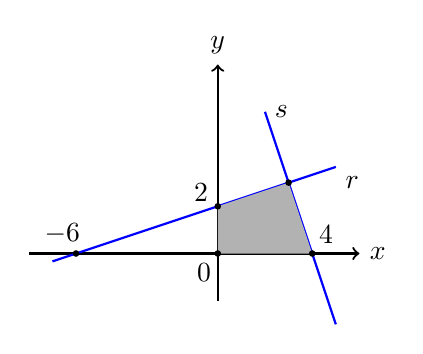
\begin{tikzpicture}[scale=0.3]
        % Eixos
        \draw[->,thick] (-8,0) -- (6,0) node[right] {$x$};
        \draw[->,thick] (0,-2) -- (0,8) node[above] {$y$};

        % Retas
        \draw[domain=-7:5, smooth, variable=\x, blue, thick] 
        plot ({\x}, {\x/3+2});
        
        \draw[domain=2:5, smooth, variable=\x, blue, thick] 
        plot ({\x}, {-3*\x+12});

        % Quadrilátero sombreado
        \fill[gray!60]
        (0,0) --
        (0,2) --
        (3,3) --
        (4,0) -- cycle;

        % Marcas no eixo x
        \node[left, above, xshift=-5pt] at (-6,0) {$-6$};
        \node[left, below, xshift=-5pt] at (0,0) {$0$};
        \node[right, above, xshift=5pt] at (4,0) {$4$};

        % Marca no eixo y
        \node[left,yshift=5pt] at (0,2) {$2$};

        % Identificação das retas
        \node[right] at (5,3) {$r$};
        \node[right] at (2,6) {$s$};
        
        % Pontos importantes
        \fill (0,0) circle (4pt);
        \fill (0,2) circle (4pt);
        \fill (3,3) circle (4pt);
        \fill (4,0) circle (4pt);
        \fill (-6,0) circle (4pt);
    \end{tikzpicture}
\end{center}

% Define as alternativas
\newcommand{\alternativas}{%
    \begin{center}
        \begin{tabularx}{\textwidth}{XXXXX}
            (a) 8 u.a.. &
            (b) 9 u.a.. &
            (c) 10 u.a.. &
            (d) 11 u.a.. &
            (e) 12 u.a..
        \end{tabularx}
    \end{center}
}

% Define a resposta correta
\newcommand{\resposta}{B}

% Lógica condicional para exibição
\ifdefstring{\atividade}{lista}{%
    \alternativas
    \vspace{0.5em}
    
    \noindent\textbf{Resposta:} letra \textbf{\resposta}.
}{%
    \ifdefstring{\modo}{objetivo}{%
        \alternativas
    }{%
        % modo = discursiva → não mostra alternativas
    }
}
\end{exercicioBanco}

